%\documentclass[aps,prl,preprint,groupedaddress]{revtex4-1}
%\documentclass[aps,prl,preprint,superscriptaddress]{revtex4-1}
\documentclass[aps,prl,twocolumn,superscriptaddress]{revtex4-1}
%\documentclass[aps,pre,preprint,superscriptaddress]{revtex4-1}
%\documentclass[aps,pre,preprint,groupedaddress{revtex4-1}
\usepackage{graphicx}% Include figure files
\usepackage{dcolumn}% Align table columns on decimal point
\usepackage{bm}% bold math
\usepackage[centertags]{amsmath}
\usepackage{amsfonts}
\usepackage{amssymb}
\usepackage{amsthm}
\usepackage{newlfont}
\usepackage{color}
\usepackage{natbib}
\usepackage{subfigure}

 
\begin{document}

\title{Fast and Accurate Determination of Phase Transition Temperature in Computer Simulation}

\author{Mingzhe Shao}
\affiliation{Department of Packaging and Printing, Tianjin University of Science and Technology, Tianjin, China}

\author{Xin Zhou$^{*}$}
\affiliation{School of Physical Sciences, University of Chinese Academy of Sciences, Beijing 100049 China}

\date{\today}
 

\begin{abstract}  
Generalized canonical ensemble (GCE) simulations are performed in water/ice coexisting systems to obtain its phase transition temperature. For the first time, the equilibrium at water/ice coexisting state can be studied in an individual simulation. This equilibrium, no longer a stochastic process, leads to a remarkable increase in both efficiency and accuracy of determining melting points. In this study, TIP4P/2005, TIP4P/ICE, mW water model are applied to build Ice Ih/water two-phase systems, then equilibrated at distinct areas in energy surface. States such as bulk water, ice and water/ice coexisting have been evolved, and their corresponding temperature are gained at the same time. The result of phase transition temperature is in excellent agreement with previous studies, is 253K, 272K, and 274K, respectively. Results from small systems show subtle accuracy lost.  These features make GCE approach determining phase transition temperature robust, easy to use, and particularly good at working on computationally expensive systems.
\end{abstract}

\pacs{ } 

\maketitle{}
\section{Introduction}

The transition between different molecular structures induce significant changes in physical properties.  However, these changes are not yet well understood in many transitions, their mechanism at the molecular level remains largely unknown.
exp1:The transition between the ferromagnetic and paramagnetic phases of magnetic materials at the Curie point.
exp2:transition into superconductive state.
exp3: Hydrogen bonding between individual water molecules yields a disordered three-dimensional hydrogen-bond network whose rugged and complex global potential energy surface permits a large number of possible network configurations, ~\cite{Matsumoto2002} making water freezing one of the most intriguing phase transition system. 
These issues call forth more comprehensive knowledge of phase transition, especially the details in multiple-phased systems (MPS). During last decades, many molecular model based molecular dynamic(MD) and Monte-Carlo (MC) simulations have been successfully applied to study thermodynamics and kinetics in MPS, offering novel and a more thorough perspectives\cite{Conde2017,Gao2000,Molinero2009,Moore2011,Sanz2004a,Sanz2004,Smit1992} . 

Estimating the molecular model corresponding transitional temperature has been a long term issue. Take the TIP4P water model as example, it is proposed by Jorgensen in 1983\cite{Jorgensen1983} and well performs in revealing the density of liquid water, density near critical point and enthalpy of vaporization\cite{Vega2011}.  A rough estimate of melting point of Ice Ih is first given by Kroes\cite{Kroes1992} as  $230K<T_m<250K$, by monitoring translational mobility of atoms on the ice/water interfaces. Later in 2000, with free energy(FE) calculation, Gao indicates $T_m=238 \pm$7 K\cite{Gao2000}.  While another study with FE approach proposed by Vega in 2005 implies a similar result, $T_m=232 \pm$5 K\cite{Vega2005}.  Although the FE approach determined phase transitional temperature is theoretically flawless, refers to the state at which two phases have Gibbs free energy identical, tiny statistical error in free energy estimation can lead to a totally different result. Gao describe this as "1 percent in relative error lead to a shift of melting point more than 10K"\cite{Gao2000}, FE approach seems to reach its limit. 

Direct coexistence(DC) simulations in MPS is also a generally accepted method to determine the phase transition temperature, this method is particularly popular in extracting the gas-liquid coexisting line on the phase diagram with canonical ensembles\cite{Ghoufi2008b,Vega2007,Alejandre1995,Ladd1977Triple}, and also can be applied in liquid/solid systems\cite{Conde2017,Bryk2002,Conde2013}.These works of determining phase transitional temperature with DC approach show great agreement with FE approach, and sometimes better presicion if the data sample sufficient. For example, with a reparametrization of TIP4P water model TIP4P-2005\cite{Abascal2005a}, Conde calculate its melting point for Ice Ih in both FE and DC approach, that is, $252\pm$5 and $249\pm$3, respectively\cite{Conde2013}. In 2017, by performing simulations covered a range of temperature space, repeating the simulation with different seeds for 5 times, using the potential energy evolution in tens of nanoseconds as phase transition indicating order parameter, Conde develop the DC approach with exhaustive study, obtaining $T_m=249.5\pm0.1$ with best precision to date. However, it is cpu-cost expensive and not so convinent.

In this work, we aim to provide a simple method of high-precision and efficiency for determining the phase transition temperature in MPS. To achieve such goal, generalized canonical ensemble (GCE)\cite{Xu2012,Xu2015} has been implemented successfully in ice Ih/water MPS with mW, TIP4P-2005, TIP4P-ICE water models and Lennard-Jones(LJ) paritcles. GCE can sufficiently visit the phase-coexistence regions and its energy distribution can be Gaussian-like, making one or several single simulations of DC approach enough to estimate phase transition temperature. Besides the enhanced sampling in GCE expanded sample volume insure considerable precision of estimation.

This work is organized as follows: Sec. II describes the models and methodology used in this work. Section III presents the results for MPS for different models. The papers ends with a final discussion and the conclusions of this work.
\section{Models and Methods} 
\subsection{A. Models}
TIP4P-2005 and TIP4P-ICE water model, two popular choice are selected to assess our method. Another two simple single-particle models are used, as well. One is the Lennard-Jones particle, the other is the mW water model. mW water is a coarse-grained model\cite{Molinero2009} using Stillinger-Weber potential to describe the tetrahedral hydrogen bond network in water and ice has been developed to accelerate the computation. In this paper, melting temperature of the proton disordered Ice Ih is obtained with three water models, while melting temperature of fcc solid for LJ particles. Thus verify our method in determining phase transition temperature. 

%In Table\ref{table:water model}  we present the geometry and the potential parameters of two popular potential full atom water models used in this work. 
\subsection{B. Simulation Details}
In our work, system is built with 32480 or 4584 water molecules for mW (approximately $400 \AA \times 56 \AA \times 43 \AA$) and full atom water model (approximately $200 \AA \times 26 \AA \times 29 \AA$), respectively. Ice phase is extract from 20ns equilibrated bulk ice Ih at 260K, with x-y plane set as ice Ih basal plane, leaving the secondary prismatic plane ($1\overline{2}10$) in contact with bulk water. The two phases system are equilibrated for another 100 ps to produce the interfaces. The size in x direction is about 7 time of y and z direction, to ensure stable interfaces and study size effect in measuring phase transition temperature. For LJ model, 8200 fcc solid and 8000 liquid coexisting system is performed in a similar way.

All MD simulations were carried out in GCE embeded isothermal–isobaric(NPT) ensembles, employing LAMMPS molecular dynamics code with GCE module\cite{Xu2012}. A Nose-Hoover barostat\cite{Hoover1985} with  relaxation times 1 ps are used to keep the pressure fixed at 1atm. For full atom water model, a time step of 2\,fs  was used in all simulations. Lennard-Jones interactions are truncated smoothly at 13.0 Å. Nontruncated electrostatic interactions are treated by the particle-particle particle mesh solver (pppm) with a real space cutoff of 13.0 Å and precision tolerance of $10^{-5}$.  The mW water is built by following previous work of Molinero and co-workers\cite{Molinero2009}. The LJ system using a cutoff of 2.5$\sigma$

\section{Results and Discussion} 
The direct coexistence technique is to put in contact two or more phases in one simulation box and study its thermodynamics. In our work, we still build our system in such classic way to clarify the effect induced by crystal lattice and interfacial crystal plane. And of course, save computational cost especially in freezing of full atom water. Water/ice coexisting systems are balanced at 250K for 100 ps, these short simulations are not enough for system to attain equilibrium, but able to relax the interfaces and a energy value $H=E+PV$ for NPT or $E$ for NVT ensemble can be extract to guide setting  energy value of GCE simulations\cite{Xu2012,Xu2015}. For mW ice Ih/water case, this value is around $-10.7 kcal/mol$  ,  the GCE equilibrated conformation with energy value range from $-9.9$ to $-11.5$ are shown in Fig\ref{fig:conformation}. Since water/ice transition involves no significant volume change, the energy value identifies the numerical average of water and ice energy, a lower energy value means more ice content. It is quite the same with unusal NPT ensemble if the equilibrated conformation is bulk phase, since energy distribution in bulk phase is always unimodal. That is, when H = -9.9,-10.1,-11.5 , GCE ensembles act like NPT ensemble of bulk water at 312K, 286K and bulk ice at 268K, as the evolutions of GCE ensembles  shown in Fig.\ref{fig:evolution}.
\begin{figure}[ht]
\centering{}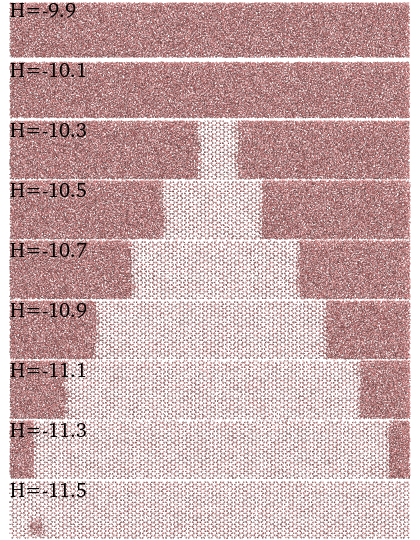
\includegraphics[width=0.5\textwidth]{conf.png} 
\caption{The conformations of GCE ensembles at distinct energy levels: From bulk water above room temperature to completely freezed ice Ih.
\label{fig:conformation} }
\end{figure}

It takes a comparably short time (less than 2ns) for mW water to attain equilibrium. However, data between 5ns to 60ns are  sampled to generate its statistical average. Only former 5ns data is presented in Fig.\ref{fig:evolution} to focus on the equilibrating temperature of 6 distinct MPS(H range form $-11.3$ to $-10.3 kcal/mol$) spontaneously evolve into one value(~275.1K). This phenomenon is self-consistent, does not rely on initial setting, thus making this GCE approach very adaptive. In Fig. \ref{fig:PTtemp-mw}, we compare the temperature of GCE ensembles with referred melting point $274.6\pm 1K$  \cite{Molinero2009} (color in cyan), the result shows good agreement. With six sample covered the water/ice coexisting system energy space, we extract the statistical average $T_m=275.1\pm0.3K$.
\begin{figure}[ht]
\centering{}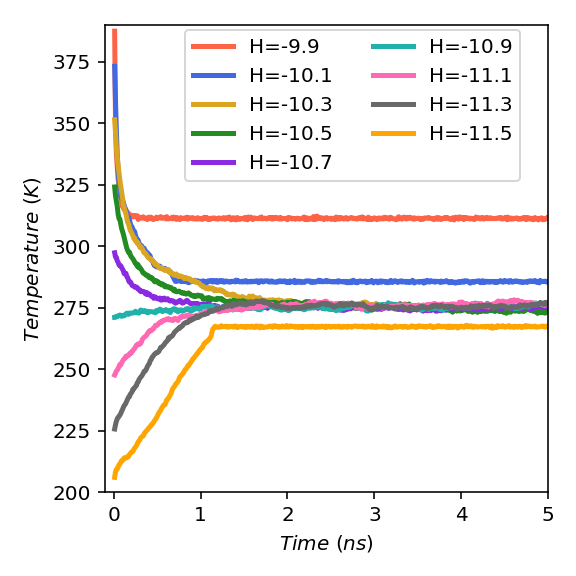
\includegraphics[width=0.5\textwidth]{PoteScan.png} 
\caption{The evolution of GCE ensembles at distinct energy levels: Starting with a ice Ih/water coexisting state. Only the former 5ns equilibrium is plotted.
\label{fig:evolution} }
\end{figure}
It has to be point out, melting point we extract from GCE ensembles of distinct energy level slightly differs. With four models applied in this study shown in Fig.\ref{fig:PTtemp-mw}-\ref{fig:PTtemp-ICE} we obtained a slightly but however affirmatively decrease of the phase transitional temperature while the melting going on. This trend shows good agreements with previous work from Sanz and Vega\cite{Sanz2013}, indicating larger critical nucleus calls for a higher critical temperature. We looking forward a more comprehensive work to elucidate this effect in the future. In spite of this, this work determined the transition temperature of MPS as the statistical average of samples covering coexisting system energy space.

 \begin{figure}[ht]
\centering{}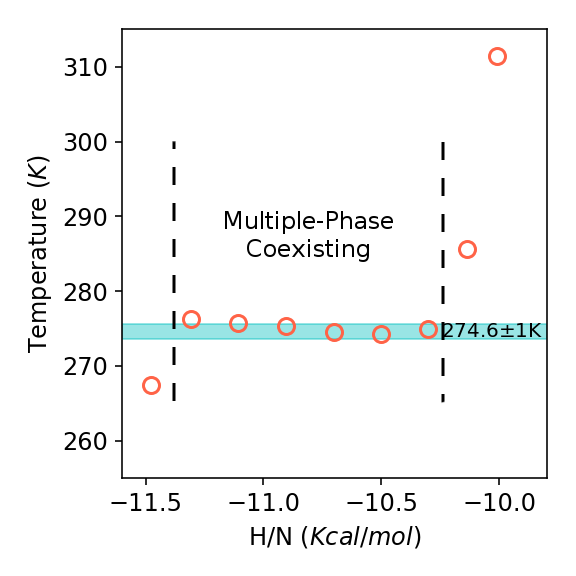
\includegraphics[width=0.5\textwidth]{PTtemp-mw.png} 
\caption{The phase transition temperature in GCE ensembles. cyan region refers to $274.6\pm1K$, the melting point for mW water proposed in previous study \cite{Molinero2009}. $T_m=275.1\pm0.3K$ is the statistical result of six systems located in the multiple-phase coexisting region.
\label{fig:PTtemp-mw}} 
\end{figure}

This approach is also tested with full-atom water models and LJ models as shown in Table. \ref{tab:tab1}. In order to save expensive cpu cost, smaller MPS composed of 4584 water molecules are applied in full-atom water systems, and run for 40ns at most to collect trajectories. This time scale is not very sufficient for the MPS to attain equilibrium, especially in highly supercooled MPS case, since the growth rate is proportional to the diffusivity of supercooled liquid water\cite{Tanaka2003}. However, the results still outline a rough but explicit picture of this GCE method. Once the MPS is built, simulations covering the energy space of multiple-phase coexisting state will spontaneously reveal the phase transitional temperature. For TIP4P-2005 water model, the result is $250.0\pm0.6K$, match with $T_m(DC)=249\pm3K$, $T_m(FE)=252\pm5K$ and $T_m(DC)=249.5\pm0.1K$ from previous research\cite{Conde2013,Conde2017}. The TIP4P-ICE water model have a better performance in generating ice/water phase diagram, our result $T_m=270.2\pm0.3K$ shows an excellent consistency with documents\cite{Conde2017,Abascal2005}. As a well studied simple model in molecular dynamics simulation, The triple point temperature of LJ particles is known as $T^*=0.617\epsilon/k_B$, showing excellent agreement with our result  $T_m=0.619\pm0.003\epsilon/k_B$. 

\newcommand{\tabincell}[2]{\begin{tabular}{@{}#1@{}}#2\end{tabular}}  

\begin{table}
\caption{Melting points Tm of the mW, TIP4P/2005, TIP4P/Ice water and LJ models as obtained from different methodologies (free energy calculations, direct coexistence technique and grand-canonical ensemble approach).}

\centering{}%
\begin{tabular}{ccccc}
%\toprule 
\hline
{ Method} & {mW} & {TIP4P-2005}  & {TIP4P-ICE}  & {LJ} \tabularnewline
%\midrule
\hline
{ FE} & { $274.6\pm1$\cite{Molinero2009}} & {$252\pm6$\cite{Abascal2005}}  & {$272\pm6$\cite{Abascal2005}}  & {0.617\cite{Broughton1986}} \tabularnewline
\hline
{ DC} & { - } & \tabincell{c}{$249\pm3$\cite{Conde2013}\\$249.5\pm0.1$\cite{Conde2017}} & \tabincell{c}{$268\pm2$\cite{GarciaFernandez2006}\\$269.8\pm0.1$\cite{Conde2017}}  & {-}  \tabularnewline
\hline
{ GCE} & { $275.1\pm0.3$} & {$250.0\pm0.6$ }  &{$270.2\pm0.3$} & {$0.619\pm0.003$} \tabularnewline
\hline
\end{tabular}
\label{table:tab1}
\end{table}


To further explore the performance of this approach, we carried out more simulations of different system size. Three GCE ensembles of 44800, 5971, 2030 water molecules are built  to apply the strategy, with size approximately $151\AA \times  156 \AA \times  58 \AA$, $54 \AA \times  58 \AA \times  58 \AA$, $52\AA \times  56 \AA \times  22\AA$ respectively.  Their result is colored in red in Fig. \ref{fig:sizeeffect},  which is $275.08\pm 0.32$, $275.00\pm 0.42$, and $275.21\pm 0.56$, while the black one $275.15\pm 0.3$ is the data presented in Fig. \ref{fig:PTtemp-mw}. The size of error bar largely depends on how many MPS we applied to cover the  energy space of coexisting state, cause such plat surfaces can be very unstable since the energy barrier to transform into a spherical cluster is relatively small, leading to fewer samples of stable MPS in small system(6,6,4,3 respectively for these four systems). Despite of this, even in the smallest system of 2030 molecules, its precision of melting temperature is still very considerable. This implies that the precision of GCE method determined phase transitional temperature not necessarily relies on the size of simulation box. A fine and close scan in the energy space over phase coexisting state can also helps to increase the precision. This feature makes GCE approach determining phase transition temperature of high precision, and in a very fast and easy-to-use manner.

\begin{figure}[ht]
\centering{}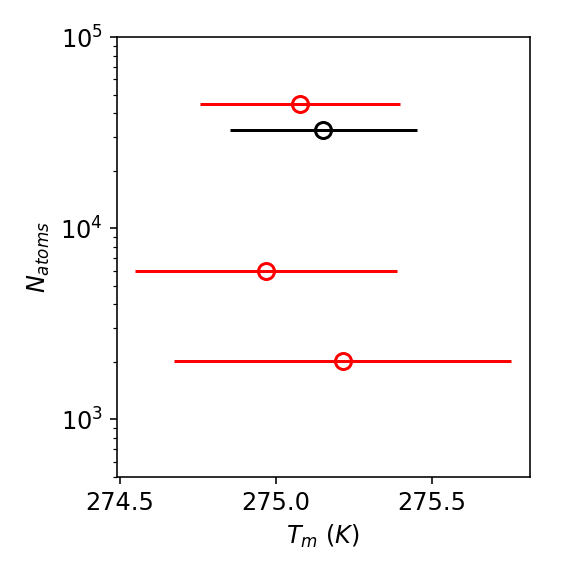
\includegraphics[width=0.5\textwidth]{size_effect.png} 
\caption{Size effect in GCE method determined phase transition temperature. Data from Fig.\ref{fig:PTtemp-mw} is plot in black, the other data is extract from GCE of 44800, 5971, 2030 water molecules, with size approximately $151\AA \times  156 \AA \times  58 \AA$, $54 \AA \times  58 \AA \times  58 \AA$, $52\AA \times  56 \AA \times  22\AA$,respectively.
\label{fig:sizeeffect}} 
\end{figure}
 
%\section{Conclusions} 
It has been found that GCE approach is very applicable of sampling metastable state, as we did in this work sampling MPS in water freezing and LJ solid melting. By following a classic direct coexistence simulation technique, GCE method can be applied to obtain its corresponding temperature to locate the MPS to the setting energy space. This temperature is the phase transitional temperature if a multiple-phase coexisting state energy level is set. Precision of this approach is considerable and does not necessarily rely on system size. Results of mW, tip4p-2005, tip4p-ice water and LJ models show good agreements with references. This novel method is robust, fast and easy-to-use.
    
%\section{Acknowledgement} 
The work is under the financial support of the NSFC Grant with No. 11574310, 11674345. C.-L. Wang thanks the support of the Youth Innovation Promotion Association, CAS. 

%%%END OF MAIN TEXT%%%

\bibliography{gce-PTtemp}
%You need to replace "rsc" on this line with the name of your .bib file
%\bibliographystyle{rsc} %the RSC's .bst file

\end{document}